\documentclass{scrreprt}

\usepackage{aligned-overset}
\usepackage{amsmath}
\usepackage{amsthm}
\usepackage{amssymb}
\usepackage{bm}
\usepackage[inline, shortlabels]{enumitem}
\usepackage{hyperref}
\usepackage[utf8]{inputenc}
\usepackage{listings}
\usepackage{multicol}
\usepackage{mathtools}
\usepackage{pdflscape}
\usepackage{physics}
\usepackage{polynom}
\usepackage{tabularx}
\usepackage[table]{xcolor}
\usepackage{titling}
\usepackage{fancyhdr}
\usepackage{xfrac}
\usepackage{pgfplots}

\pgfplotsset{compat = newest}
\usepgfplotslibrary{fillbetween}
\usetikzlibrary{arrows, arrows.meta}
\usetikzlibrary{calc}
\usetikzlibrary{patterns}

\author{Karsten Lehmann}
\date{WiSe 2024/25}
\title{Übungsblatt 11\\INF-B-110, Diskrete Strukturen}

\setlength{\parindent}{0pt}

\setlength{\headheight}{26pt}
\pagestyle{fancy}
\fancyhf{}
\lhead{\thetitle}
\rhead{\theauthor}
\lfoot{\thedate}
\rfoot{Seite \thepage}

\newcommand{\ggT}[0]{\text{ggT}}
\DeclarePairedDelimiter{\floor}{\lfloor}{\rfloor}

\begin{document}

\paragraph{Ü 11.1} \phantom{\null}

\begin{minipage}{0.7\textwidth}
  Durch nebenstehendes Diagramm ist ein Graph
  $G = \qty\big(V, E)$ gegeben.
  Es werden die Knotenmengen $A = \qty\big{2, 3, 4, 5}$ und
  $B = \qty\big(6, 7, 8, 9)$ betrachtet.
  \begin{enumerate}[(a)]
  \item Bestimmen Sie die maximale Anzahl disjunkter $A$-$B$-Pfade in $G$ und
    eine minimale Menge $X \subseteq V$, die $A$ und $B$ in $G$ trennt.

  \item Finden Sie die maximale Zahl $k \in \mathbb{N}$, so dass $G$ $k$-fach
    zusammenhängend ist.
  \end{enumerate}
\end{minipage}
\begin{minipage}{0.2\textwidth}
  \begin{tikzpicture}
    \node[circle, draw, inner sep=0pt, minimum size=1mm,label=above:{1}] (1) at (0,0) {};
    \node[circle, draw, inner sep=0pt, minimum size=1mm,label=above:{2}] (2) at (1,0) {};
    \node[circle, draw, inner sep=0pt, minimum size=1mm,label=right:{3}] (3) at (2,-0.8) {};
    \node[circle, draw, inner sep=0pt, minimum size=1mm,label=right:{4}] (4) at (2.3,-2) {};
    \node[circle, draw, inner sep=0pt, minimum size=1mm,label=right:{5}] (5) at (1.5,-3) {};
    \node[circle, draw, inner sep=0pt, minimum size=1mm,label=below:{6}] (6) at (0.5,-3.5) {};
    \node[circle, draw, inner sep=0pt, minimum size=1mm,label=left:{7}] (7) at (-0.5,-3) {};
    \node[circle, draw, inner sep=0pt, minimum size=1mm,label=left:{8}] (8) at (-1.3,-2) {};
    \node[circle, draw, inner sep=0pt, minimum size=1mm,label=left:{9}] (9) at (-1,-0.8) {};
    \node[circle, draw, inner sep=0pt, minimum size=1mm,label=above:{10}] (10) at (0.5,-2) {};

    \draw (1) -- (4) -- (3) -- (2) -- (8) -- (9) -- (1) -- (5) -- (4);
    \draw (1) -- (9) -- (8) -- (7) -- (6) -- (5);
    \draw (2) -- (7);
    \draw (6) -- (10) -- (3);
    \draw (9) -- (10);
  \end{tikzpicture}
\end{minipage}

\subparagraph{Lsg.}
\begin{enumerate}[(a)]
\item  Es sind \colorbox{green!20}{$A$} und \colorbox{red!20}{$B$}
  eingefärbt:

  \begin{tikzpicture}
    \node[circle, draw, inner sep=0pt, minimum size=1mm,label=above:{1}] (1) at (0,0) {};
    \node[circle, draw, fill, black!20!green, inner sep=0pt, minimum size=1mm,label={[color=black!30!green] above:{2}}] (2) at (1,0) {};
    \node[circle, draw, fill, black!20!green, inner sep=0pt, minimum size=1mm,label={[color=black!30!green] right:{3}}] (3) at (2,-0.8) {};
    \node[circle, draw, fill, black!20!green, inner sep=0pt, minimum size=1mm,label={[color=black!30!green] right:{4}}] (4) at (2.3,-2) {};
    \node[circle, draw, fill, black!20!green, inner sep=0pt, minimum size=1mm,label={[color=black!30!green] right:{5}}] (5) at (1.5,-3) {};
    \node[circle, draw, fill, black!20!red, inner sep=0pt, minimum size=1mm,label={[color=black!30!red] below:{6}}] (6) at (0.5,-3.5) {};
    \node[circle, draw, fill, black!20!red, inner sep=0pt, minimum size=1mm,label={[color=black!30!red] left:{7}}] (7) at (-0.5,-3) {};
    \node[circle, draw, fill, black!20!red, inner sep=0pt, minimum size=1mm,label={[color=black!30!red] left:{8}}] (8) at (-1.3,-2) {};
    \node[circle, draw, fill, black!20!red, inner sep=0pt, minimum size=1mm,label={[color=black!30!red] left:{9}}] (9) at (-1,-0.8) {};
    \node[circle, draw, inner sep=0pt, minimum size=1mm,label=above:{10}] (10) at (0.5,-2) {};

    \draw (1) -- (4) -- (3) -- (2) -- (8) -- (9) -- (1) -- (5) -- (4);
    \draw (1) -- (9) -- (8) -- (7) -- (6) -- (5);
    \draw (2) -- (7);
    \draw (6) -- (10) -- (3);
    \draw (9) -- (10);
  \end{tikzpicture}

  Es ist die minimale Menge $X \subseteq V$, die \colorbox{green!20}{$A$} von
  \colorbox{red!20}{$B$} trennt
  \[
    X = \qty\big{
      \colorbox{green!20}{$2$},
      \colorbox{red!20}{$6$},
      \colorbox{red!20}{$9$}
    }
  \]
  (Die Menge muss minimal sein, da sich leicht 3 disjunkte
  \colorbox{green!20}{$A$}-\colorbox{red!20}{$B$}-Pfade $\qty\big{5, 6}$,
  $\qty\big{2, 8}$ und $\qty\big{3, 10, 9}$ finden)

  Somit ist die maximale Anzahl an paarweise disjunkten $A$-$B$-Pfaden in $G$ nach
  dem Satz von Menger gleich $\abs{X} = 3$.

\item Der Graph ist schon mal nicht 4-fach zusammenhängend, da in Teilaufgabe
  (a) eine Menge mit 3 Elementen gefunden wurde, die den Graphen trennt.

  Allerdings ist der Graph 3-fach zusammenhängend, durch Probieren erkennt man,
  dass er nach Entnahme zweier beliebiger Knoten immer noch zusammenhängt.

  \textbf{Nach der Übung:} Es soll an der Aufgabe gezeigt werden, dass es
  tatsächlich sehr Mühsam ist, denn $k$-fachen Zusammenhang zu zeigen.
  Im gegebenen Graphen ist dies nur durch Ausprobieren möglich.
\end{enumerate}

\newpage
\paragraph{Ü 11.2}
\begin{enumerate}[(a)]
\item Zeichnen Sie je ein Diagramm der Kantengraphen für die Graphen $K_{2,3}$,
  $C_5$ und $\overline{C}_4$.

  \subparagraph{Lsg.} \phantom{\null}

  \begin{minipage}{0.45\textwidth}
    Der Graph $K_{2, 3}$:

    \begin{tikzpicture}
      \node[circle, draw, inner sep=0pt, minimum size=2mm, label=left:{1}] (1) at (0,1.5) {};
      \node[circle, draw, inner sep=0pt, minimum size=2mm, label=left:{2}] (2) at (0,-1.5) {};
      \node[circle, draw, inner sep=0pt, minimum size=2mm, label=below:{3}] (3) at (1.5,-1.5) {};
      \node[circle, draw, inner sep=0pt, minimum size=2mm, label=right:{4}] (4) at (3,-1.5) {};
      \node[circle, draw, inner sep=0pt, minimum size=2mm, label=right:{5}] (5) at (3,1.5) {};

      \draw (1) -- (2) -- (5) -- (4) -- (1) -- (3) -- (5);
    \end{tikzpicture}
  \end{minipage}
  \begin{minipage}{0.45\textwidth}
    Und der zugehörige Katengraph:

    \begin{tikzpicture}
      \node[circle, draw, inner sep=0pt, minimum size=2mm, label=above:{$\qty\big{4, 5}$}] (1) at (0,1) {};
      \node[circle, draw, inner sep=0pt, minimum size=2mm, label=left:{$\qty\big{3, 5}$}] (2) at (-2,2) {};
      \node[circle, draw, inner sep=0pt, minimum size=2mm, label=below:{$\qty\big{1, 3}$}] (3) at (-2,-1) {};
      \node[circle, draw, inner sep=0pt, minimum size=2mm, label=below:{$\qty\big{1, 2}$}] (4) at (2,-1) {};
      \node[circle, draw, inner sep=0pt, minimum size=2mm, label=right:{$\qty\big{2, 5}$}] (5) at (2,2) {};
      \node[circle, draw, inner sep=0pt, minimum size=2mm, label=below:{$\qty\big{1, 4}$}] (6) at (0,0) {};

      \draw (1) -- (2) -- (3) -- (4) -- (5) -- (1) -- (6) -- (3);
      \draw (6) -- (4);
      \draw (2) -- (5);
    \end{tikzpicture}
  \end{minipage}

  \begin{minipage}{0.45\textwidth}
    Der Graph $C_5$:

    \begin{tikzpicture}
      \node[circle, draw, inner sep=0pt, minimum size=2mm, label=above:{1}] (1) at (0,1) {};
      \node[circle, draw, inner sep=0pt, minimum size=2mm, label=left:{2}] (2) at ($({-sqrt(0.5*(5+sqrt(5)))/2}, {sqrt(5)/4 - 0.25})$) {};
      \node[circle, draw, inner sep=0pt, minimum size=2mm, label=below:{3}] (3) at ($({-sqrt(0.5*(5-sqrt(5)))/2}, {-0.25 - sqrt(5)/4})$) {};
      \node[circle, draw, inner sep=0pt, minimum size=2mm, label=below:{4}] (4) at ($({sqrt(0.5*(5-sqrt(5)))/2}, {-0.25 - sqrt(5)/4})$) {};
      \node[circle, draw, inner sep=0pt, minimum size=2mm, label=right:{5}] (5) at ($({sqrt(0.5*(5+sqrt(5)))/2}, {sqrt(5)/4 - 0.25})$) {};

      \draw (1) -- (2) -- (3) -- (4) -- (5) -- (1);
    \end{tikzpicture}
  \end{minipage}
  \begin{minipage}{0.45\textwidth}
    Und der zugehörige Katengraph:

    \begin{tikzpicture}
      \node[circle, draw, inner sep=0pt, minimum size=2mm, label=above:{$\qty\big{1, 5}$}] (1) at (0,1) {};
      \node[circle, draw, inner sep=0pt, minimum size=2mm, label=left:{$\qty\big{5, 4}$}] (2) at ($({-sqrt(0.5*(5+sqrt(5)))/2}, {sqrt(5)/4 - 0.25})$) {};
      \node[circle, draw, inner sep=0pt, minimum size=2mm, label=below:{$\qty\big{4, 3}$}] (3) at ($({-sqrt(0.5*(5-sqrt(5)))/2}, {-0.25 - sqrt(5)/4})$) {};
      \node[circle, draw, inner sep=0pt, minimum size=2mm, label=below:{$\qty\big{3, 2}$}] (4) at ($({sqrt(0.5*(5-sqrt(5)))/2}, {-0.25 - sqrt(5)/4})$) {};
      \node[circle, draw, inner sep=0pt, minimum size=2mm, label=right:{$\qty\big{2, 1}$}] (5) at ($({sqrt(0.5*(5+sqrt(5)))/2}, {sqrt(5)/4 - 0.25})$) {};

      \draw (1) -- (2) -- (3) -- (4) -- (5) -- (1);
    \end{tikzpicture}
  \end{minipage}

  \begin{minipage}{0.45\textwidth}
    Der Graph $\overline{C}_4$:

    \begin{tikzpicture}
      \node[circle, draw, inner sep=0pt, minimum size=2mm, label=above left:{1}] (1) at (0,0) {};
      \node[circle, draw, inner sep=0pt, minimum size=2mm, label=above right:{2}] (2) at (1,0) {};
      \node[circle, draw, inner sep=0pt, minimum size=2mm, label=below right:{3}] (3) at (1,-1) {};
      \node[circle, draw, inner sep=0pt, minimum size=2mm, label=below left:{4}] (4) at (0,-1) {};

      \draw (1) -- (3);
      \draw (2) -- (4);
    \end{tikzpicture}
  \end{minipage}
  \begin{minipage}{0.45\textwidth}
    Und der zugehörige Katengraph:

    \begin{tikzpicture}
      \node[circle, draw, inner sep=0pt, minimum size=2mm, label=above left:{$\qty\big{1, 3}$}] (1) at (0,0) {};
      \node[circle, draw, inner sep=0pt, minimum size=2mm, label=above right:{$\qty\big{2, 4}$}] (2) at (2,0) {};
    \end{tikzpicture}
  \end{minipage}

\item Zeigen Sie: Ist $G$ ein zusammenhängender Graph, dann ist auch der
  Kantengraph $L\qty\big(G)$ zusammenhängend.
  Gilt auch die Umkehrung dieser Aussage?

  \paragraph{Lsg.} Seien $u, v$ zwei beliebige Knoten in $V\qty(L\qty\big(G))$.
  Nach der Definition des Kantengraphes gibt es dann
  $a = \qty\big{a_1, a_2}, b = \qty\big{b_1, b_2} \in E\qty\big(G)$, die $u$ und
  $v$ entsprechen.
  Nun ist $G$ zusammenhängend, dass heißt es gibt einen minimalen Pfad von $a_1$
  nach $b_1$ in der Form $\qty\big(a_1, v_1, \ldots, v_n, b_1)$ mit
  $v_1, \ldots, v_n \in V\qty\big(G)$.

  Nun sind $\qty\big{a_1, v_1}$, $\qty\big{v_1, v_2}$, $\ldots$,
  $\qty\big{v_n, b_1}$ alle Kanten in $E\qty\big{G}$ und somit Knoten in
  $L\qty\big(G)$.
  Da jeweils genau zwei dieser Gruppen ein gemeinsames Element haben, existieren
  auch entsprechende Kanten in $L\qty\big(G)$ und somit ein Pfad zwischen $u$
  und $v$.
  Da $u$ und $v$ beliebig folgt die Behauptung.

  Die Umkehrung gilt hingegen nicht.
  Betrachten wir den nicht-zusammenhängenden Graphen $H$

  \begin{tikzpicture}
    \node[circle, draw, inner sep=0pt, minimum size=2mm, label=below:{1}] (1) at (0,0) {};
    \node[circle, draw, inner sep=0pt, minimum size=2mm, label=below:{2}] (2) at (1,0) {};
    \node[circle, draw, inner sep=0pt, minimum size=2mm, label=below:{3}] (3) at (2,0) {};
    \node[circle, draw, inner sep=0pt, minimum size=2mm, label=below:{4}] (4) at (3,0) {};

    \draw (2) -- (3) -- (4);
  \end{tikzpicture}

  dann ist dessen Kantengraph $L\qty\big(H)$ zusammenhängend:

  \begin{tikzpicture}
    \node[circle, draw, inner sep=0pt, minimum size=2mm, label=below:{$\qty\big{2, 3}$}] (1) at (0,0) {};
    \node[circle, draw, inner sep=0pt, minimum size=2mm, label=below:{$\qty\big{3, 4}$}] (2) at (1,0) {};

    \draw (2) -- (1);
  \end{tikzpicture}
\end{enumerate}

\paragraph{Ü 11.3} Es sei $G = \qty\big(V, E)$ ein Graph und es bezeichne
$d_G\qty\big(v)$ die Anzahl Kanten, die den Knoten $v$ enthalten, d.h. den
Knotengrad von $v$.
Zeigen Sie, dass die Anzahl der Kanten von $L\qty\big(G)$ gleich
\[
  \frac{1}{2}\sum_{v \in V}\qty(d_G\qty\big(v))^2 - \abs{E}
\]
ist.
Überprüfen Sie die Formel zuerst am Graphen $K_{2, 3}$.

\subparagraph{Lsg.} Der Graph $K_{2, 3}$ und sein Kantengraph:

\begin{minipage}{0.45\textwidth}
  \begin{tikzpicture}
    \node[circle, draw, inner sep=0pt, minimum size=2mm, label=above:{1}] (1) at (0,1.5) {};
    \node[circle, draw, inner sep=0pt, minimum size=2mm, label=left:{2}] (2) at (0,-1.5) {};
    \node[circle, draw, inner sep=0pt, minimum size=2mm, label=below:{3}] (3) at (1.5,-1.5) {};
    \node[circle, draw, inner sep=0pt, minimum size=2mm, label=right:{4}] (4) at (3,-1.5) {};
    \node[circle, draw, inner sep=0pt, minimum size=2mm, label=above:{5}] (5) at (3,1.5) {};

    \draw (1) -- (2) -- (5) -- (4) -- (1) -- (3) -- (5);

    \node at (1.5, -2.5) {$K_{2, 3}$};
  \end{tikzpicture}
\end{minipage}
\begin{minipage}{0.45\textwidth}
  \begin{tikzpicture}
    \node[circle, draw, inner sep=0pt, minimum size=2mm, label=above:{$\qty\big{4, 5}$}] (1) at (0,1) {};
    \node[circle, draw, inner sep=0pt, minimum size=2mm, label=left:{$\qty\big{3, 5}$}] (2) at (-2,2) {};
    \node[circle, draw, inner sep=0pt, minimum size=2mm, label=below:{$\qty\big{1, 3}$}] (3) at (-2,-1) {};
    \node[circle, draw, inner sep=0pt, minimum size=2mm, label=below:{$\qty\big{1, 2}$}] (4) at (2,-1) {};
    \node[circle, draw, inner sep=0pt, minimum size=2mm, label=right:{$\qty\big{2, 5}$}] (5) at (2,2) {};
    \node[circle, draw, inner sep=0pt, minimum size=2mm, label=below:{$\qty\big{1, 4}$}] (6) at (0,0) {};

    \draw (1) -- (2) -- (3) -- (4) -- (5) -- (1) -- (6) -- (3);
    \draw (6) -- (4);
    \draw (2) -- (5);

    \node at (0.5, -2) {$L\qty(K_{2, 3})$};
  \end{tikzpicture}
\end{minipage}

Nun hat der Graph $K_{2, 3}$ 6 Kanten und
\begin{itemize}
\item $d_G\qty\big(1) = 3$
\item $d_G\qty\big(2) = 2$
\item $d_G\qty\big(3) = 2$
\item $d_G\qty\big(4) = 2$
\item $d_G\qty\big(5) = 3$
\end{itemize}
Somit ist
\[
  \frac{1}{2}\sum_{v \in V}\qty(d_G\qty\big(v))^2 - \abs{E} =
  \frac{1}{2}\qty(2 \cdot 3^2 + 3 \cdot 2^2) - 6 =
  9
\]
und das ist offensichtlich korrekt.
Wie kommt diese Formel nun zustande?

Sei $k = \qty\big(a, b) \in E$ eine Kante in $G$.
Dann sind $a, b \in V$ Knoten aus $G$ und die Existenz der Kante $k$ erhöht sowohl
den Grad von $a$ als auch von $b$ um jeweils eins.
Somit ist $\abs{E} = \frac{1}{2}\sum_{v \in V}d_G\qty\big(v)$.

Sei nun jeder Knoten in $e \in E\qty(L\qty\big(G))$ als $e = \qty\big{c, d}$
wobei $c$ und $d$ die beiden Knoten in $G$ sind, welche die Kante, die $e$
erzeugt begrenzen.
Dann hat per Definition des Kantengraphens jede Kante in $L\qty\big(G)$ die
Form $\qty{\qty\big{a, b}, \qty\big{b, c}}$ und der Kante lässt sich eindeutig
ein Knoten aus $G$ zuordnen, nämlich das Element, welches in beiden Mengen
vorhanden ist.

Wie viele Kanten in $L\qty\big(G)$ erzeugt nun ein Knoten aus $G$?
Nun soviele, wie man zwei aus seine Kanten ohne Zurücklegen oder Beachtung der
Reihenfolge auswählen kann.
Somit ist die Zahl der Kanten in $L\qty\big(G)$
\begin{flalign*}
  \sum_{v \in V} \binom{d_G\qty\big(V)}{2}
  &= \sum_{v \in V} \frac{d_G\qty\big(v)!}{2\qty\big(d_G\qty\big(v) - 2)!} \\
  &= \sum_{v \in V} \frac{d_G\qty\big(v)\qty(d_G\qty\big(v) - 1)d_G\qty\big(v) - 2)!}{2\qty\big(d_G\qty\big(v) - 2)!} \\
  &= \sum_{v \in V} \frac{d_G\qty\big(v)\qty(d_G\qty\big(v) - 1)}{2} \\
  &= \frac{1}{2}\sum_{v \in V} d_G\qty\big(v)^2 - d_G\qty\big(v) \\
  &= \frac{1}{2}\sum_{v \in V} d_G\qty\big(v)^2 - \frac{1}{2} \sum_{v \in V} d_G\qty\big(v) \\
  &= \frac{1}{2}\sum_{v \in V} d_G\qty\big(v)^2 - \abs{E}
\end{flalign*}

\newpage
\paragraph{Ü 11.4} \phantom{\null}

\begin{minipage}{0.3\textwidth}
  \begin{tikzpicture}
    \node[circle, draw, inner sep=0pt, minimum size=2mm] (1) at (0,1) {};
    \node[circle, draw, inner sep=0pt, minimum size=2mm] (2) at (0,-1) {};
    \node[circle, draw, inner sep=0pt, minimum size=2mm] (3) at (1.5,-1) {};
    \node[circle, draw, inner sep=0pt, minimum size=2mm] (4) at (3,-1) {};
    \node[circle, draw, inner sep=0pt, minimum size=2mm] (5) at (3,1) {};

    \draw (1) -- (2) -- (5) -- (4) -- (1) -- (3) -- (5);

    \node at (1, -1.5) {$G_1$};
  \end{tikzpicture}
\end{minipage}
\begin{minipage}{0.3\textwidth}
  \begin{tikzpicture}
    \node[circle, draw, inner sep=0pt, minimum size=2mm] (1) at (0,1) {};
    \node[circle, draw, inner sep=0pt, minimum size=2mm] (2) at ($({-sqrt(0.5*(5+sqrt(5)))/2}, {sqrt(5)/4 - 0.25})$) {};
    \node[circle, draw, inner sep=0pt, minimum size=2mm] (3) at ($({-sqrt(0.5*(5-sqrt(5)))/2}, {-0.25 - sqrt(5)/4})$) {};
    \node[circle, draw, inner sep=0pt, minimum size=2mm] (4) at ($({sqrt(0.5*(5-sqrt(5)))/2}, {-0.25 - sqrt(5)/4})$) {};
    \node[circle, draw, inner sep=0pt, minimum size=2mm] (5) at ($({sqrt(0.5*(5+sqrt(5)))/2}, {sqrt(5)/4 - 0.25})$) {};


    \draw (1) -- (2) -- (3) -- (4) -- (5) -- (1) -- (3) -- (5) -- (2) -- (4) -- (1);

    \node at (0, -2) {$G_2$};
  \end{tikzpicture}
\end{minipage}
\begin{minipage}{0.3\textwidth}
  \begin{tikzpicture}
    \node[circle, draw, inner sep=0pt, minimum size=2mm] (1) at (0,1) {};
    \node[circle, draw, inner sep=0pt, minimum size=2mm] (2) at (0,-1) {};
    \node[circle, draw, inner sep=0pt, minimum size=2mm] (3) at (1,-1) {};
    \node[circle, draw, inner sep=0pt, minimum size=2mm] (4) at (1,1) {};
    \node[circle, draw, inner sep=0pt, minimum size=2mm] (5) at (2,1) {};
    \node[circle, draw, inner sep=0pt, minimum size=2mm] (6) at (2,-1) {};
    \node[circle, draw, inner sep=0pt, minimum size=2mm] (7) at (3,-1) {};
    \node[circle, draw, inner sep=0pt, minimum size=2mm] (8) at (3,1) {};

    \draw (4) -- (1) -- (2) -- (3) -- (4) -- (6) -- (7) -- (8) -- (5) -- (6);
    \draw (1) -- (3) -- (5) -- (7);
    \draw (6) -- (8);
    \draw (2) -- (4);

    \node at (1, -1.5) {$G_3$};
  \end{tikzpicture}
\end{minipage}

\begin{enumerate}[(a)]
\item Gibt es in den durch Diagramme gegebenen Graphen offene oder geschlossene
  Eulerzüge?

  \subparagraph{Lsg.} Nach Satz 75 der Vorlesung hat ein zusammenhängender
  endlicher Graph genau dann einen geschlossenen Eulerzug, wenn jeder seiner
  Knoten einen geraden Grad hat.
  Nun hat $G_1$ zwei Knoten mit Grad 3 und besitzt somit keinen geschlossenen
  Eulerzug.

  Allerdings einen offenen Eulerzug:

  \begin{tikzpicture}
    \node[circle, draw, inner sep=0pt, minimum size=2mm] (1) at (0,1) {};
    \node[circle, draw, inner sep=0pt, minimum size=2mm] (2) at (0,-1) {};
    \node[circle, draw, inner sep=0pt, minimum size=2mm] (3) at (1.5,-1) {};
    \node[circle, draw, inner sep=0pt, minimum size=2mm] (4) at (3,-1) {};
    \node[circle, draw, inner sep=0pt, minimum size=2mm] (5) at (3,1) {};

    \draw (5) -- (2) -- (1) -- (3) -- (3, 0.7) -- (4) -- (0.2, 0.9);
  \end{tikzpicture}


  $G_2$ hat einen geschlossenen Eulerzug:

  \begin{tikzpicture}
    \node[circle, draw, inner sep=0pt, minimum size=2mm] (1) at (90:2) {};
    \node[circle, draw, inner sep=0pt, minimum size=2mm] (2) at (18:2) {};
    \node[circle, draw, inner sep=0pt, minimum size=2mm] (3) at (306:2) {};
    \node[circle, draw, inner sep=0pt, minimum size=2mm] (4) at (234:2) {};
    \node[circle, draw, inner sep=0pt, minimum size=2mm] (5) at (162:2) {};


    \draw (1) -- (2) -- (3) -- (4) -- (5) -- (90:1.7) -- (306:1.7) -- (162:1.7) -- (18:1.7) -- (234:1.7) -- (95:1.4);
  \end{tikzpicture}

  Und $G_3$ hat wieder Knoten mit ungeradem Grad, also keinen geschlossenen Eulerzug.
  Weiter besitzt nach Satz 76 der Vorlesung ein Graph genau daunn einen offenen
  Eulerzug, wenn er genau zwei Knoten mit ungeradem Grad hat.
  Da $G_4$ 4 Knoten mit Grad 3 besitzt, hat der Graph auch keinen offenen Eulerzug.

\newpage
\item Für welches maximale $k \in \mathbb{N}$ sind die einzelnen Graphen $k$-fach
  zusammenhängend?

  \subparagraph{Lsg.} Der Graph $G_2 = \qty(V_2, E_2)$ enthält für alle
  $a, b \in V_2$ genau 4 paarweise unabhängige Pfade von $a$ nach $b$ und ist
  somit nach Satz 67 der Vorlesung 4-fach zusammenhängend.
  (5-facher Zusammenhang ist nicht geben, da der Graph dafür nach der Definitio
  des $k$-fachen Zusammenhangs $k + 1$ Knoten bräuchte).

  Analog ist $G_1$ zweifach zusammenhängend.

  $G_3$ hat eine Engstelle in der Mitte mit 2-Pfaden.
  Durch Anwendung von Satz 67 ist auch er 2-fach zusammenhängend.
\end{enumerate}

\paragraph{Ü 11.5}
\begin{enumerate}[(a)]
\item Für ein beliebiges, fest gewähltes $n \in \mathbb{N}, n > 0$ wird der Graph
  $G_n$ mit Knotenmenge $V = \qty\big{a_1, \ldots, a_n, b_1, \ldots, b_n}$ und
  den Kanten $\qty\big{a_k, b_k}, k = 1, \ldots, n$ und
  $\qty\big{a_k, a_{k + 1}}$ und $\qty\big{b_k, b_{k + 1}}, k = 1, \ldots, n$
  betrachtet.
  Finden Sie eine rekursive Formel für die Anzahl perfekter Paarungen $G_n$.

  \subparagraph{Lsg.} Betrachten wir den Graphen $G_1$ mit
  $V_1 = \qty\big{a_1, b_1}$ und $E_1 = \qty{\qty\big{a_1, b_1}}$.
  Der Graph hat zwei Paarungen
  \begin{itemize}
  \item $\emptyset$ - nicht perfekt
  \item $E_1$ - perfekt.
  \end{itemize}

  ... den Graphen $G_2$ mit $V_2 = \qty\big{a_1, a_2, b_1, b_2}$ und
  $E_2 = \qty{
    \qty\big{a_1, b_1},
    \qty\big{a_2, b_2},
    \qty\big{a_1, a_2},
    \qty\big{b_1, b_2}
  }$
  Der Graph hat zwei perfekte Paarungen
  \begin{itemize}
  \item $\qty{\qty\big{a_1, b_1}, \qty\big{a_2, b_2}}$
  \item $\qty{\qty\big{a_1, a_2}, \qty\big{b_1, b_2}}$
  \end{itemize}

  ... den Graphen $G_3$ mit $V_3 = \qty\big{a_1, a_2, a_3, b_1, b_2, b_3}$ und \\
  $E_2 = \qty{
    \qty\big{a_1, b_1},
    \qty\big{a_2, b_2},
    \qty\big{a_3, b_3},
    \qty\big{a_1, a_2},
    \qty\big{a_2, a_3},
    \qty\big{b_1, b_2},
    \qty\big{b_2, b_3}
  }$

  Der Graph hat drei perfekte Paarungen
  \begin{itemize}
  \item $\qty{\qty\big{a_1, b_1}, \qty\big{a_2, b_2}, \qty\big{a_3, b_3}}$
  \item $\qty{\qty\big{a_1, a_2}, \qty\big{b_1, b_2}, \qty\big{a_3, b_3}}$
  \item $\qty{\qty\big{a_2, a_3}, \qty\big{b_2, b_3}, \qty\big{a_1, b_1}}$
  \end{itemize}

  \newpage
  Allgemein hat der Graph $G_n$ die Form

  \begin{tikzpicture}
    \node[circle, draw, inner sep=0pt, minimum size=2mm, label=above:{$a_1$}] (a1) at (0,0) {};
    \node[circle, draw, inner sep=0pt, minimum size=2mm, label=below:{$b_1$}] (b1) at (0,-1) {};
    \node[circle, draw, inner sep=0pt, minimum size=2mm, label=above:{$a_2$}] (a2) at (1.5,0) {};
    \node[circle, draw, inner sep=0pt, minimum size=2mm, label=below:{$b_2$}] (b2) at (1.5,-1) {};
    \node[circle, draw, inner sep=0pt, minimum size=2mm, label=above:{$a_3$}] (a3) at (3,0) {};
    \node[circle, draw, inner sep=0pt, minimum size=2mm, label=below:{$b_3$}] (b3) at (3,-1) {};
    \node[circle, draw, inner sep=0pt, minimum size=2mm, label=above:{$a_4$}] (a4) at (4.5,0) {};
    \node[circle, draw, inner sep=0pt, minimum size=2mm, label=below:{$b_4$}] (b4) at (4.5,-1) {};
    \node[circle, draw, inner sep=0pt, minimum size=2mm, label=above:{$a_{n-2}$}] (an2) at (7,0) {};
    \node[circle, draw, inner sep=0pt, minimum size=2mm, label=below:{$b_{n-2}$}] (bn2) at (7,-1) {};
    \node[circle, draw, inner sep=0pt, minimum size=2mm, label=above:{$a_{n-1}$}] (an1) at (8.5,0) {};
    \node[circle, draw, inner sep=0pt, minimum size=2mm, label=below:{$b_{n-1}$}] (bn1) at (8.5,-1) {};
    \node[circle, draw, inner sep=0pt, minimum size=2mm, label=above:{$a_n$}] (an) at (10,0) {};
    \node[circle, draw, inner sep=0pt, minimum size=2mm, label=below:{$b_n$}] (bn) at (10,-1) {};

    \draw (a1) -- (b1);
    \draw (a2) -- (b2);
    \draw (a3) -- (b3);
    \draw (a4) -- (b4);
    \draw (an2) -- (bn2);
    \draw (an1) -- (bn1);
    \draw[black!10!red, line width=1mm] (an) -- (bn);

    \draw (a1) -- (a2) -- (a3) -- (a4);
    \draw (b1) -- (b2) -- (b3) -- (b4);

    \draw[dashed] (a4) -- (an2);
    \draw[dashed] (b4) -- (bn2);

    \draw (an2) -- (an1);
    \draw (bn2) -- (bn1);
    \draw[black!10!blue, line width=1mm] (an1) -- (an);
    \draw[black!10!blue, line width=1mm] (bn1) -- (bn);
  \end{tikzpicture}

  Nun ergeben sich die Perfekten Paarungen von $G_n$ indem man entweder den
  perfekten Paarungen von $G_{n - 1}$ die Kante
  \colorbox{red!20}{$\qty\big{a_n, b_n}$} hinzufügt, denn diese ist zu allen
  Kanten aus $G_{n - 1}$ disjunkt, oder den perfekten Paarungen aus $G_{n - 2}$
  die Kanten \colorbox{blue!20}{$\qty\big{a_{n - 1}, a_n}$} und
  \colorbox{blue!20}{$\qty\big{b_{n - 1}, b_n}$} anfügt - diese sind ebenfalls
  zu allen Kanten aus $G_{n - 2}$ disjunkt.
  Somit ist die Anzahl der perfekten Paarungen
  \[
    P_n = P_{n - 1} + P_{n - 2}
  \]
  Also die Fibonacci-Folge.

\item Es sei $G = \qty\big(V, E)$ ein Graph und $M \subseteq E$ eine Paarung für
  $G$.
  Wir betrachten die Relation
  \[
    R_M = \qty{\qty\big(u, v) \in V \times V \:\middle|\: \exists e \in M \colon u \in e, v \in e}
  \]
  Untersuchen Sie, für welche $M$ die Relation $R_M$ eine Äquivalenzrelation ist
  und geben Sie in diesem Fall $V \setminus R_M$ an.

  \subparagraph{Lsg.} $R_M$ ist eine Äquivalenzrelation, falls $R_M$
  \emph{reflexiv}, \emph{transitiv} und \emph{symmetrisch} ist.

  \begin{itemize}
  \item[\emph{reflexiv}] Die Relation ist reflexiv, falls für alle $v \in V$ gilt
    $\qty\big(v, v) \in R_M$.
    Auf die Relation umformuliert
    \[
      \forall v \in V \exists e \in M \colon v \in e
    \]
    Somit existiert für jeden Knoten auch eine Kante, die diesen Knoten enthält
    in der Paarung $M$.

    $\Rightarrow M$ muss eine perfekte Paarung sein

  \item[\emph{transitiv}] Die Relation ist transitiv, wenn für drei Knoten
    $u, v, w \in V$ gilt
    \[
      \qty\big(u, v), \qty\big(v, w) \in R_M \Rightarrow \qty\big(u, w) \in R_M
    \]
    Da nun $M$ eine Paarung ist, kommt jeder Punkt in maximal einer Kante in $M$
    vor.
    Somit folgt
    \[
      \exists e \in M \colon u \in e, v \in e \land
      \exists e' \in M \colon v \in e', w \in e'
      \Rightarrow e = e'
    \]
    und auch $\qty\big(u, w) \in R_M$.

  \item[\emph{symmetrisch}] Die Relation ist symmetrisch, wenn für alle
    $u, v \in V$ gilt
    \[
      \qty\big(u,v) \in R_M \iff \qty\big(v,u) \in R_m
    \]
    und das ist trivial.
  \end{itemize}

  $\Rightarrow$ Die Relation $R_M$ ist genau dann eine Äquivalenzrelation, wenn
  $M$ eine perfekte Paarung ist.

  Nun ist $V / R_M = M$.
\end{enumerate}
\end{document}
